Both the EM and online learning methods for training the recurrent deep GSN have their drawbacks - EM only models the sequence linearly in the latent variable \(H\) space while the online learning method requires untied weights between layers. This model, the hybrid approach, aims to combine the best of both worlds by creating an alternating structure inspired by convolutional neural networks with alternating convolutional and pooling layers \cite{lenet5}.

\section{Generalizing the EM model}
The EM model is easier to train and appears to have better mixing in both the input and sequence spaces compared to the online learning model. However, due to the simple regression step, it is unable to represent complex sequences in the representation space. A more general model is necessary to encode complex data in both input and representation spaces.

Ultimately, this model generalizes Model 1 by alternating between finding a good representation for inputs and a good representation for sequences. This way, the GSNs can optimize specifically for reconstruction or prediction rather than making the hidden representation learn both. Further, by making the sequence prediction GSN layer recurrent over the top layer of the input reconstruction GSN layer, this system can learn complex, nonlinear sequence representations over the modes of the input space, capturing a very large possibility of sequential data distributions. These two specified layers can then be repeated to form deep, generalized representations of sequential data.


\section{Algorithm}
This algorithm also alternates between training the reconstruction GSN parameters and prediction GSN for transitions.
 \begin{algorithm}[h!]
	\KwIn{training data \(X\) from a sequential distribution \(D\)}
	Initialize reconstruction GSN parameters \(\Theta_{reconstruction} = \) \{List(weights from one layer to the next), List(bias for layer))\}\;
	Initialize transition GSN parameters \(\Theta_{transition} = \) \{List(weights from one layer to the next higher), List(weights from on layer to the next lower), List(bias for layer))\}\;
	\While{training not converged}{
		\For{each input \(X\)}{
			Sample from reconstruction GSN with walkback using \(X\) to create \((X_{recon},X)\) pairs for training parameters \(\Theta_{reconstruction}\)\;
			Sample from transition GSN using the hidden representations \(H\) from the reconstruciton GSN on the input \(X\)\;
			Store the predicted next hidden representations \(H'\) and use them with sampling from the next reconstruction GSN to train the transition parameters \(\Theta_{transition}\)\;
			Perform sequential walkback training on the transition GSN\;
		}
	}
	\caption{ Model 3 Hybrid  Recurrent Deep GSN Algorithm }
\end{algorithm}


\section{Experimental results}
Model 3 uses the same general training parameters with regards to noise, learning rate, annealing, momentum, epochs, hidden layers, and activation as Model 1 and Model 2. In addition, it has one recurrent hidden layer of 3000 units, receiving input from layer 1 and layer 3 of the GSN below it. No sequential walkback steps were performed. Model 3 performed worse with regards to binary cross-entropy of the predicted reconstruction than models 1 and 2 (achieving a score of 0.2695, with the current reconstruction achieving a score of 0.1669). However, the reconstruction and predicted reconstruction after 300 training iterations qualitatively looks like the model is learning the correct sequence. Further, because of the additional recurrent layer and parameters, this model should take longer to train and slower progress to sequence prediction is expected. Further study of this general model should be with hyper-parameter optimization and more training epochs.

\begin{figure}[h!]
  \centering
    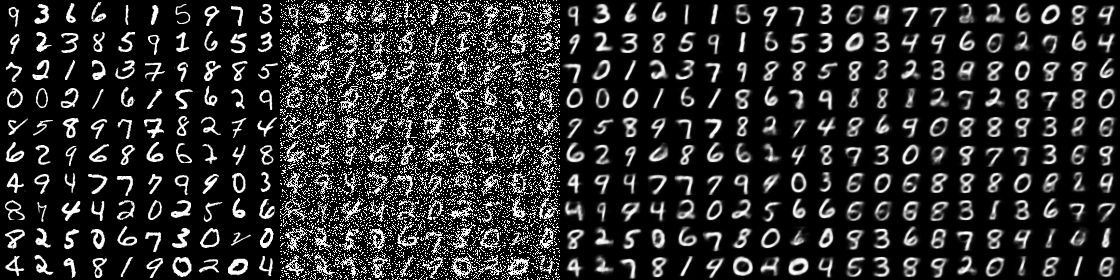
\includegraphics[width=1.0\textwidth]{story3_reconstruction}
\caption{Model 3 reconstruction of current digits and predicted next digits after 300 iterations.}
\end{figure}

The sampling is only pulled from the first GSN layer, so it looks similar to Model 1 with regards to mixing between modes of the input space.
\begin{figure}[h!]
  \centering
    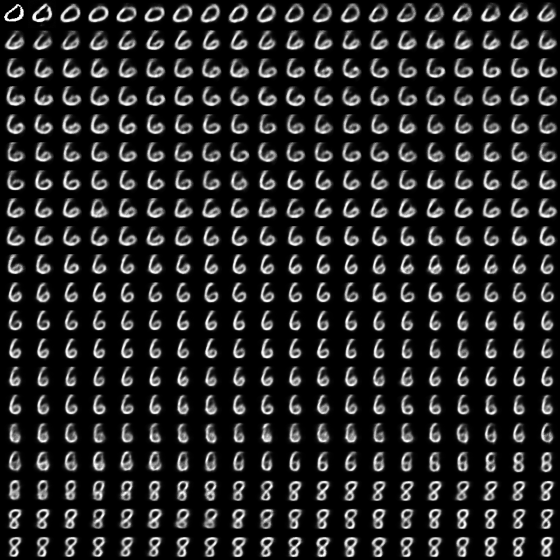
\includegraphics[width=.8\textwidth]{story3_samples_170}
\caption{Model 2 sampling after 300 iterations.}
\end{figure}